\subsection{Legacy Precision Under Strong Updates}\label{app:legacy_precision}

The strong-update policy in Appendix~\ref{app:early_update} sends
$90\%$ of examples to the exact old suffix. We first test narrowing
the old block while retaining its skip path and output gate. A
head-independent student distils the teacher's activations and pooled
features on $12{,}000$ unlabeled image views. Intermediate widths
$64$, $128$, and $256$ require $80\%$, $70\%$, and $50\%$ referral on
both development monitors. The width-$256$ path reaches the query
target with an old-block MAC proxy of one. All widths miss the joint
development criterion.

Precision gives a separate option with the original channel widths.
We calibrate static x86 INT8 observers on $1{,}024$ unlabeled prefix
tensors. The selected program evaluates the two old convolutions in
INT8 and retains FP32 residual addition, the output gate, pooling and
the old affine reader. Its maximum monitor disagreements are $0.98\%$
and $1.17\%$. Quantizing the skip and output gate gives $0.59\%$ and
$1.37\%$. The BF16 convolution control gives $0.20\%$ on both.
The fixed priority selects INT8 with the FP32 skip.

We reconstruct the six strong continuations and seal both old-output
programs before accessing the official test batch. Each reference
uses a disjoint $1{,}500$-image partition. The previous terminal-feature
policy calls the exact old block on $90.6\%$ of test inputs after batch
rounding. The selected INT8 program calls it on none. Its largest
class or threshold disagreement across all six references is
$1.73\%$, within the $5\%$ budget. Both programs use the same FP32
current predictions. The INT8 program evaluates the complete
low-precision old block on each input. It takes only the frozen prefix
and fitted legacy reader, so replacing the trainable suffix leaves
this approximate legacy function unchanged for a fixed batch.

We time four programs on the same CPU batches with a shared FP32
current graph. Each reference uses $12$ warmups and $31$ interleaved
passes at batch $128$. The INT8 program costs $1.043\times$
$[1.036,1.050]$ relative to current-only, compared with $1.187\times$
$[1.175,1.200]$ for the prior referral program and $1.185\times$
$[1.171,1.199]$ for the exact two-output program. The paired INT8
ratio is $0.878$ $[0.874,0.883]$ relative to prior referral and
$0.880$ $[0.875,0.886]$ relative to exact two-output serving.
Intervals use six reference ratios.

\begin{figure}[H]
\centering
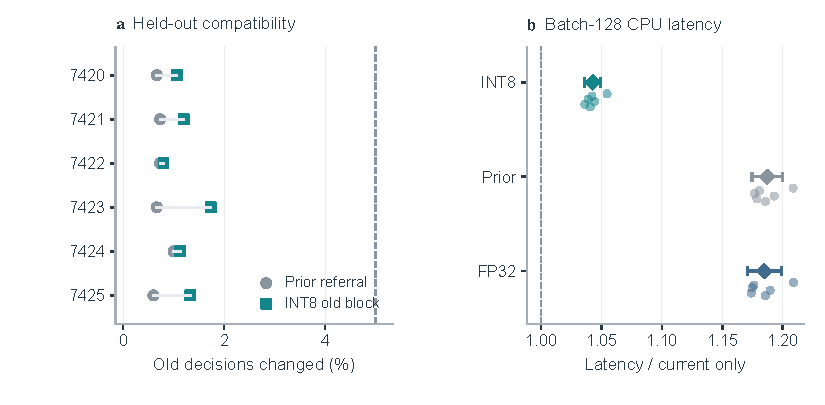
\includegraphics[width=\linewidth]{figures/fig_legacy_precision.pdf}
\caption{A low-precision legacy block under strong continuation.
(a) Maximum class or threshold disagreement on six disjoint CIFAR-10
test partitions. The prior program refers $90.6\%$ of inputs to the
exact old block. INT8 uses zero exact calls. (b) Physical CPU latency
with a shared FP32 current graph. Points are reference ratios.
Diamonds show means and paired $95\%$ intervals.}
\label{fig:legacy_precision}
\end{figure}
